\section{Approximation von Funktionen}
Da die Approximation von Funktionen nicht zu den gew�hnlichen Aufgaben eines Elman Netzes geh�rt, habe ich versucht eine Funktion mit dem selben Netz, welches bei der System Identification verwendet wurde, zu approximieren. Das hei�t, es wurde die selbe Architektur (Abbildung \ref{arche}), der selbe Lernparameter $\eta = 0,7$, die selbe Aktivierungsfunktion $\varphi(x) = \frac{1}{1+e^{-x}}$ und die gleich Menge an 100 Input- und Outputwerten verwendet. Als die zu approximierende Funktion w�hlte ich
$$e^{-\frac{x}{4}} \cos x.$$
Diese Funktion wird in Abbildung \ref{function} dargestellt.
\begin{figure}[H]
	\centering
	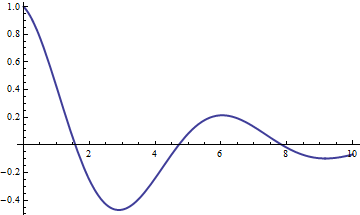
\includegraphics[height=6cm]{func.png}
	\caption{Funktion}
	\label{function}
\end{figure} 

Nach 100 Epochen meines Netzes erhalte ich folgende Gegen�berstellung (Abbildung \ref{result3}), wobei die blaue Linie die zu approximierende Funktion und die violetten Punkte den Netzoutput darstellen.
\begin{figure}[H]
	\centering
	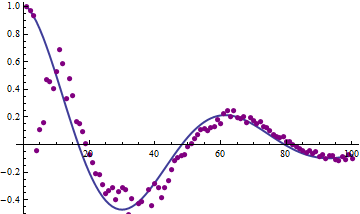
\includegraphics[height=6cm]{approx.png}
	\caption{Approximation}
	\label{result3}
\end{figure}

\section{Fazit}
Wie die Gegen�berstellung zeigt, ist die Approximation noch nicht ausgereift und man kann mit einer anderen Architektur eventuell bessere Werte erzielen. Au�erdem ist diese Gegen�berstellung ein Ausnahmebeispiel meines Netzes und nicht alle 100 Epochen wurden so gute Ergebnisse getroffen. Der Gesamtfehler liegt hier bei $E = 1,3207026786535492$, wobei der Gesamtfehler der System Identification unter $0,2$ liegt. Abschlie�end kann man sagen, dass das Problem der System Identification mittels der durch die dynamische Backpropagation trainierten Elman Netze gute Ergebnisse erzielt und f�r die Funktionenapproximation gr��ere Fehler aufweist.
